% !TeX program = pdflatex
% -------------------------------------------------------------------------
%  crowbar_thyristor_selftrigger.tex
%  Crowbar thyristor for the 3 kV / 3600 A static-switch test bench:
%  device selection and passive self-triggering gate circuit.
%  Rev. 01: simulated load-voltage waveform, trigger level, detailed sizing.
%  Conventions: English, thebibliography (no biblatex), no babel, no lmodern.
%  Figures: load_voltage.pdf (simulation, user), gate_response.pdf
%  (generated by gate_network_sim.py).
% -------------------------------------------------------------------------
\documentclass[11pt,a4paper]{article}

\usepackage[T1]{fontenc}
\usepackage[utf8]{inputenc}
\usepackage[margin=25mm]{geometry}
\usepackage{amsmath,amssymb}
\usepackage{siunitx}
\usepackage{booktabs}
\usepackage{graphicx}
\usepackage{caption}
\usepackage[european]{circuitikz}
\usepackage{fancyhdr}
\usepackage[hidelinks]{hyperref}

% ---------------- document identification / revision ----------------------
\newcommand{\doctitle}{Crowbar Thyristor for the 3~kV / 3600~A Static-Switch Test Bench}
\newcommand{\docsubtitle}{Device Selection and Passive Self-Triggering Gate Circuit}
\newcommand{\docrev}{03}
\newcommand{\docdate}{2026-09-11}
\newcommand{\docid}{crowbar\_thyristor\_selftrigger}

\pagestyle{fancy}
\fancyhf{}
\lhead{\small \docid}
\rhead{\small Rev.~\docrev}
\lfoot{\small \docdate}
\cfoot{\small \thepage}
\renewcommand{\headrulewidth}{0.4pt}

\sisetup{per-mode=symbol, range-phrase={\text{--}}, range-units=single}

\title{\textbf{\doctitle}\\[6pt]\large \docsubtitle\\[10pt]\normalsize Rev.~\docrev\ --- \docdate}
\author{}
\date{}

\begin{document}
\maketitle
\thispagestyle{fancy}

\begin{center}
\begin{tabular}{@{}llp{9.5cm}@{}}
\toprule
\textbf{Rev.} & \textbf{Date} & \textbf{Description} \\
\midrule
00 & 2026-09-09 & First issue. Device selection, stress analysis, passive gate circuit. \\
01 & 2026-09-11 & Added the simulated load-voltage waveform at breaker opening
   (Sec.~\ref{sec:uload}) and the trigger-level and sizing chapter
   (Sec.~\ref{sec:sizing}): datasheet gate data of the 5STP~26N6500, choice of the
   negative load voltage that fires the crowbar, hold capacitor for the gate pulse,
   component-by-component sizing, computed gate-current waveforms, slow-opening case,
   failure modes. Corrected the $\mathrm{d}v/\mathrm{d}t$ estimate of
   Sec.~\ref{sec:dvdt} and the turn-on sequence of Sec.~\ref{sec:network}; thyristor
   data aligned with the datasheet. \\
02 & 2026-09-11 & Added Sec.~\ref{sec:lc} on the role of the dump inductor $L_c$:
   commutation loop (Fig.~\ref{fig:loop}), why the load inductance does not limit the
   turn-on $\mathrm{d}i/\mathrm{d}t$, trade-off with the MOV energy, requirements on
   $L_c$. Conclusions updated. \\
03 & 2026-09-11 & Circuit figures (Figs.~\ref{fig:circuit}, \ref{fig:loop}, \ref{fig:gate})
   enlarged for readability; battery symbol changed. No technical change. \\
\bottomrule
\end{tabular}
\end{center}

\begin{abstract}
A thyristor crowbar with a series dump inductor and resistor extracts the energy
of a \SI{2}{mH}, \SI{3600}{A} inductive load when a \SI{3}{kV} IGBT static switch
opens. This note quantifies the electrical stress on the crowbar thyristor,
justifies the choice of a \SI{6.5}{kV} symmetric phase-control thyristor (Hitachi
Energy 5STP~26N6500), and shows that the intrinsic self-firing mechanisms of a
thyristor cannot be relied upon: with the simulated rate of rise of the load
voltage the device is in fact guaranteed \emph{not} to fire, and without a gate
circuit the varistor bank absorbs the whole load energy. A fully passive,
floating anode-to-gate network turns the reversal of the load voltage into a
regular gate pulse. Rev.~01 adds the simulated load-voltage waveform, derives from
it the negative load voltage at which the crowbar fires, and gives a complete
sizing of the network -- blocking diode, coupling capacitor, TVS stack, hold
capacitor, reset and gate-cathode elements -- against the datasheet gate data,
with computed gate-current waveforms, the slow-opening case and the failure modes.
Rev.~02 adds a section on the role of the dump inductor $L_c$: it, and not the load
inductance, sets the turn-on $\mathrm{d}i/\mathrm{d}t$, because the load inductance is
not part of the loop in which the current transfers from the varistor to the thyristor.
\end{abstract}

% ==========================================================================
\section{Scope and circuit under study}
% ==========================================================================

The circuit is the static-switch test bench of Fig.~\ref{fig:circuit}: a DC source
$V_s = \SI{3000}{V}$ feeds an RL load ($R = \SI{0.8}{\ohm}$, $L = \SI{2}{mH}$)
through an IGBT breaker $S$ (four 5SNA~1000G650300 in parallel). The breaker is
opened under load at $I_0 = \SI{3600}{A}$; a varistor bank across the breaker
clamps its voltage at $V_{\mathrm{MOV}} \approx \SI{5.5}{kV}$. The load energy is
extracted by the crowbar branch in parallel with the load: thyristor $T$, dump
inductor $L_c = \SI{12.5}{\micro H}$ and dump resistor $R_D = \SI{0.42}{\ohm}$,
with an RC snubber $C_{sn} = \SI{2}{\micro F}$, $R_{sn} = \SI{64}{\ohm}$ across the
branch. The bench must perform of the order of $10^6$ opening cycles.

The load voltage $u_{\mathrm{load}}$ is taken positive at the breaker-side terminal
of the load. The thyristor anode is on the return rail, so that before the crowbar
conducts
\begin{equation}
  v_{AK} = -\,u_{\mathrm{load}},
  \label{eq:sign}
\end{equation}
and the crowbar can conduct only when the load voltage is negative.

\begin{figure}[htbp]
\centering
\begin{circuitikz}[american, scale=1.25, transform shape]
  % source (positive terminal towards the breaker)
  \draw (0,0) to[battery2, l_=$V_s$, invert] (0,4);
  \node[font=\scriptsize] at (0.35,3.35) {$+$};
  \node[font=\scriptsize] at (0.35,0.65) {$-$};
  % breaker with MOV
  \draw (0,4) -- (1,4) to[nos, l=$S$] (3.5,4) -- (4.5,4);
  \draw (1,4) -- (1,5.5) to[varistor, l=MOV] (3.5,5.5) -- (3.5,4);
  % load
  \draw (4.5,4) -- (5.5,4) to[R, l_=$R$] (5.5,2.25) to[L, l_=$L$] (5.5,0.25) -- (5.5,0) -- (0,0);
  % load voltage arrow
  \draw[-latex] (4.7,0.9) -- (4.7,3.1);
  \node[font=\scriptsize, anchor=east] at (4.65,2.0) {$u_{\mathrm{load}}$};
  \node[font=\scriptsize] at (4.7,3.4) {$+$};
  % crowbar branch: thyristor (anode at bottom), Lc, RD
  \draw (5.5,4) -- (8,4);
  \draw (5.5,0) -- (8,0);
  \draw (8,0) to[Ty, n=T, l_=$T$] (8,1.3) to[L, l_=$L_c$] (8,2.5) to[R, l_=$R_D$] (8,4);
  % snubber across the branch
  \draw (8,4) -- (10,4) to[R, l=$R_{sn}$] (10,1.8) to[C, l=$C_{sn}$] (10,0) -- (8,0);
  % gate network box
  \draw (T.G) -- (7.15,0 |- T.G);
  \draw[dashed] (5.95,0.3) rectangle (7.15,1.9);
  \node[align=center,font=\scriptsize] at (6.55,1.1) {gate\\network\\(Fig.~\ref{fig:gate})};
  % current arrow
  \draw[-latex] (4.55,4.25) -- (5.15,4.25) node[midway, above, font=\scriptsize] {$i_L$};
\end{circuitikz}
\caption{Static-switch test bench with dump-resistor crowbar. In service ($S$ closed) the load
voltage is $+V_s$ and the thyristor blocks in the \emph{reverse} direction; forward voltage appears
across $T$ only while $S$ opens.}
\label{fig:circuit}
\end{figure}

Two facts shape the whole analysis:

\begin{enumerate}
\item In service the crowbar thyristor is \emph{reverse} biased at $-V_s = \SI{-3}{kV}$.
      Forward voltage appears only when $S$ opens and the load inductance reverses the load
      voltage, which is exactly when the crowbar must fire.
\item The forward voltage available to the crowbar is bounded by the MOV clamp of the breaker:
      \begin{equation}
        v_{AK,\max} = V_{\mathrm{MOV}} - V_s \approx \SI{5.5}{kV} - \SI{3.0}{kV} = \SI{2.5}{kV}
        \label{eq:vfw}
      \end{equation}
      as a plateau, with a first peak of about \SI{2.8}{kV} (Sec.~\ref{sec:uload}). Any firing
      threshold of the crowbar must lie well below this value, otherwise the MOV
      takes the load current and the energy.
\end{enumerate}

% ==========================================================================
\section{Load voltage at breaker opening}
\label{sec:uload}
% ==========================================================================

\subsection{Simulated waveform without crowbar}

Fig.~\ref{fig:uload} shows the load voltage simulated for a breaker opening at
$I_0 = \SI{3600}{A}$ with the MOV bank as the only energy absorber (crowbar not
firing). The features that matter for the trigger design are:

\begin{itemize}
\item The swing from $+\SI{3}{kV}$ to about $\SI{-2.5}{kV}$ is completed in roughly
      \SIrange{4}{5}{\micro s}; the maximum slope, around the zero crossing, is of the order of
      \SIrange{1.5}{2}{kV/\micro s}. This rate is set by the breaker (IGBT turn-off, its
      snubbers and the MOV loop), not by the crowbar branch.
\item The first negative peak is about \SI{-2.8}{kV}: the varistor bank clamps at its highest
      voltage while it carries the full \SI{3600}{A}, plus the drop on the loop inductance.
      The voltage then settles on the plateau $u_{\mathrm{load}} = V_s - V_{\mathrm{MOV}} \approx
      \SI{-2.5}{kV}$ and drifts to about \SI{-1.8}{kV} as the MOV current decreases.
\item The MOV conducts for about \SI{2.1}{ms}. With the MOV modelled as a constant back-voltage
      $V' = V_{\mathrm{MOV}} - V_s \approx \SI{2.3}{kV}$ the load current is
      $i(t) = (I_0 + V'/R)\,e^{-t/\tau_L} - V'/R$ with $\tau_L = L/R = \SI{2.5}{ms}$, which reaches
      zero at $t = \tau_L \ln(1 + I_0 R/V') \approx \SI{2.0}{ms}$, in agreement with the
      simulation. The energy absorbed by the varistor bank in this mode is about \SI{16.6}{kJ} per
      opening (the load energy $\tfrac12 L I_0^2 = \SI{13}{kJ}$ plus the energy delivered by the
      source during the decay, minus the part dissipated in $R$).
\item When the MOV current extinguishes, the load node rings with a positive peak of about
      \SI{+0.8}{kV}; for the thyristor this is reverse voltage and is harmless.
\end{itemize}

\begin{figure}[htbp]
\centering
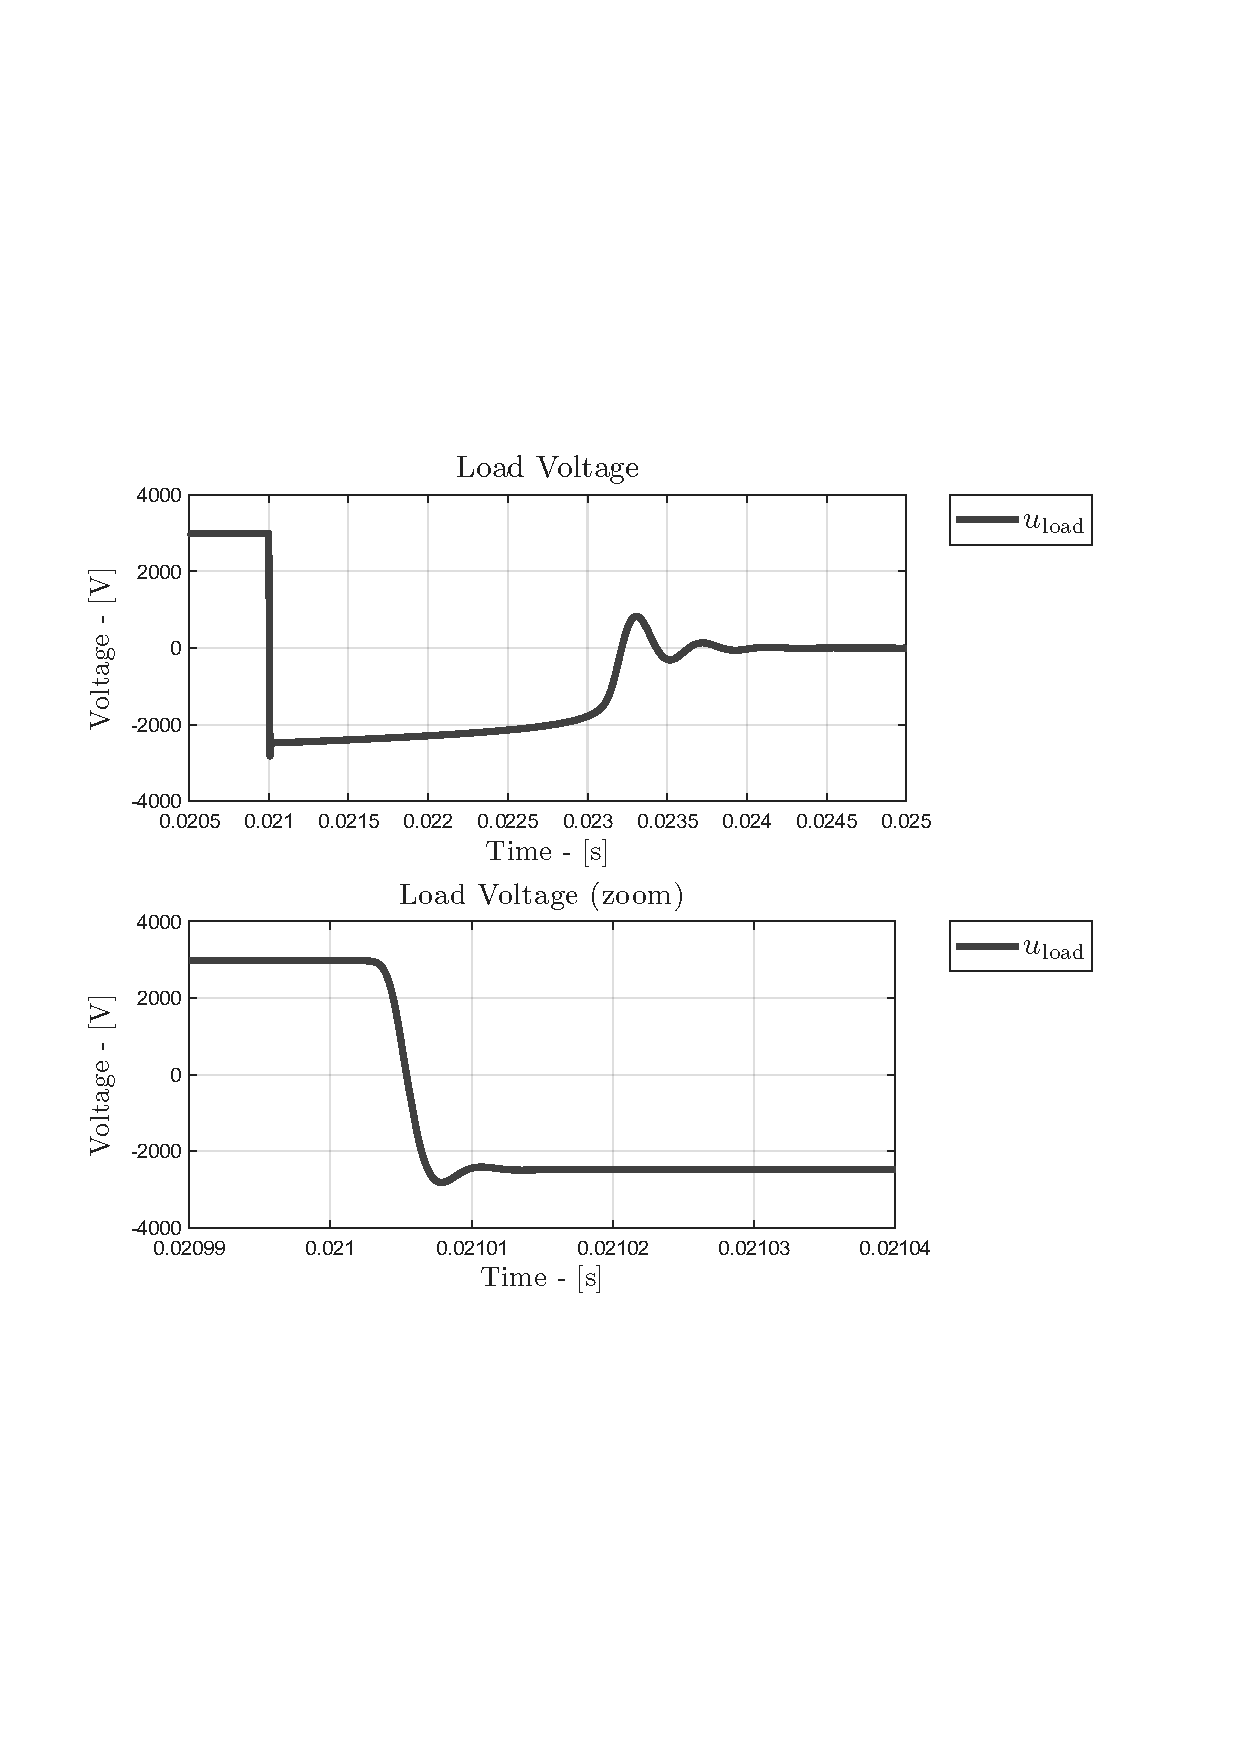
\includegraphics[width=0.82\textwidth, trim=40 205 60 200, clip]{load_voltage.pdf}
\caption{Simulated load voltage at breaker opening ($I_0 = \SI{3600}{A}$), MOV clamp only,
crowbar not firing. Top: full event; bottom: zoom on the \SI{50}{\micro s} around the opening.}
\label{fig:uload}
\end{figure}

\subsection{What the waveform means for the crowbar}
\label{sec:meaning}

\paragraph{A negative load voltage is an unambiguous ``breaker open'' signal.}
The circuit is DC and the load current is unidirectional. With the source connected,
$u_{\mathrm{load}} = V_s > 0$; during the low-voltage pre-heating phase it is still positive.
The only way for $u_{\mathrm{load}}$ to become negative is that the path from the source is
interrupted and the load inductance forces the current through whatever is left in parallel with
the load -- the MOV or the crowbar. No auxiliary logic is needed to decide when the crowbar must
fire: $u_{\mathrm{load}} < 0$, i.e.\ $v_{AK} > 0$ by \eqref{eq:sign}, is both necessary and
sufficient. The trigger network must therefore act only for $v_{AK} > 0$ and must be
completely inert for $v_{AK} < 0$; the blocking diode $D_1$ of Sec.~\ref{sec:network} does
exactly this.

\paragraph{Without a gate circuit the crowbar does not fire.}
The critical $\mathrm{d}v/\mathrm{d}t$ of the 5STP~26N6500 is \SI{3000}{V/\micro s}
(exponential to $0.67\,V_{DRM}$, $T_{vj} = \SI{125}{\celsius}$) \cite{ds26n6500}. A ramp of
\SIrange{1.5}{2}{kV/\micro s} reaching only \SI{2.8}{kV}, at a junction temperature far below
\SI{125}{\celsius}, is inside the region where the device is guaranteed not to turn on.
Forward breakover is even further away ($V_{BO} > V_{DRM} = \SI{6.5}{kV}$). A crowbar thyristor
without trigger circuit would thus behave exactly as in Fig.~\ref{fig:uload}: it would block,
and the varistor bank would absorb \SI{16.6}{kJ} at every opening. The trigger network is not a
refinement that makes the turn-on ``controlled''; it is what makes the crowbar work at all.

\paragraph{Expected waveform with the crowbar.}
With the network of Sec.~\ref{sec:network} the plateau at \SI{-2.5}{kV} lasts only for the
gate delay plus the commutation of the current into $L_c$, about $3 + 18 = \SI{21}{\micro s}$.
The load voltage then jumps to $-(R_D\,i + v_T) \approx \SI{-1.5}{kV}$ and decays exponentially
with $\tau = L/(R + R_D) = \SI{1.64}{ms}$ to zero; the MOV conducts for
\SI{20}{\micro s} and absorbs about \SI{180}{J} instead of \SI{16.6}{kJ}. This is the waveform
to be checked in the simulation once the crowbar and its network are added
(Sec.~\ref{sec:verif}).

% ==========================================================================
\section{Electrical stress on the crowbar thyristor}
% ==========================================================================

\subsection{Conduction: charge, $\int i^2\,\mathrm{d}t$, energy}

Once the load current has commutated into the crowbar branch, it decays through
$R + R_D$ with
\begin{equation}
  \tau = \frac{L}{R + R_D} = \frac{\SI{2}{mH}}{\SI{1.22}{\ohm}} \approx \SI{1.64}{ms}.
\end{equation}
The conduction quantities follow directly:
\begin{align}
  Q &= I_0\,\tau \approx \SI{5.9}{C}, \\
  \int i^2\,\mathrm{d}t &= \frac{I_0^2\,\tau}{2} \approx \SI{10.6e3}{A^2 s}, \\
  E_{L} &= \tfrac12 L I_0^2 \approx \SI{13.0}{kJ},
  \qquad E_{R_D} = E_L\,\frac{R_D}{R+R_D} \approx \SI{4.5}{kJ},
  \qquad E_{R} \approx \SI{8.5}{kJ}.
\end{align}
The thyristor conduction energy, with the on-state model $v_T = V_{T0} + r_T\,i$ of the
5STP~26N6500 ($V_{T0} = \SI{1.12}{V}$, $r_T = \SI{0.29}{m\ohm}$), is
\begin{equation}
  E_T = V_{T0}\,Q + r_T \int i^2\,\mathrm{d}t \approx 6.6 + 3.1 \approx \SI{10}{J}.
\end{equation}
Spread over the silicon of a \SI{100}{mm} wafer (thermal capacity of the order of
\SI{10}{J/K}), this gives $\Delta T_j \lesssim \SI{1}{K}$ per event. The crowbar
thyristor is therefore \emph{not} sized by current or by $\int i^2\mathrm{d}t$; it is sized by
blocking voltage, turn-on $\mathrm{d}i/\mathrm{d}t$ and cycle count. The current reaches the
holding level ($I_H = \SI{125}{mA}$ at \SI{25}{\celsius}) after $\tau\ln(I_0/I_H) \approx
\SI{17}{ms}$ and the device turns off naturally, without reverse recovery.

\subsection{Role of the dump inductor $L_c$: the commutation loop}
\label{sec:lc}

A natural objection is that the circuit already contains a large inductance, the \SI{2}{mH} of
the load, and that a further \SI{12.5}{\micro H} in the crowbar branch can hardly limit
anything. The objection misses \emph{where} the current changes. The load inductance is not
part of the loop in which the current is transferred from the breaker to the crowbar, and on
the time scale of that transfer it cannot change its current at all: with the load node at
\SI{-2.5}{kV} the load current decreases at $(V_{\mathrm{MOV}} - V_s + R I_0)/L \approx
\SI{2.7}{A/\micro s}$, i.e.\ by about \SI{50}{A} out of \SI{3600}{A} during the whole
commutation. For the commutation, $L$ is a constant current source $I_0$
(Fig.~\ref{fig:loop}).

\begin{figure}[htbp]
\centering
\begin{circuitikz}[american, scale=1.25, transform shape]
  % source
  \draw (0,0) to[battery2, l_=$V_s$, invert] (0,4);
  \node[font=\scriptsize] at (0.35,3.35) {$+$};
  \node[font=\scriptsize] at (0.35,0.65) {$-$};
  % breaker branch: S open, MOV conducting, stray inductance of the loop
  \draw (0,4) -- (1,4) to[varistor, l=MOV] (3,4) to[L, l_=$L_\sigma$] (4.3,4) -- (5.5,4);
  \draw (1,4) -- (1,5.4) to[nos, l=$S$ open] (3,5.4) -- (3,4);
  % crowbar branch (inside the loop)
  \draw (5.5,0) to[Ty, n=T, l=$T$] (5.5,1.8) to[L, l=$L_c$] (5.5,2.9) to[R, l=$R_D$] (5.5,4);
  \filldraw (5.5,4) circle (1pt);
  \filldraw (5.5,0) circle (1pt);
  % load: R + constant current source I0 (the 2 mH on the us time scale), outside the loop
  \draw (5.5,4) -- (8.5,4) to[R, l_=$R$] (8.5,2.6) to[I, l_=$I_0$] (8.5,0.6) -- (8.5,0) -- (5.5,0) -- (0,0);
  \node[font=\scriptsize, align=left, anchor=west] at (8.85,1.6) {$L = \SI{2}{mH}$:\\constant current\\on the \si{\micro s} scale};
  % currents
  \draw[-latex] (4.35,4.3) -- (5.05,4.3) node[midway, above, font=\scriptsize] {$i_{\mathrm{MOV}} = I_0 - i_c$};
  \draw[-latex] (6.9,4.3) -- (7.6,4.3) node[midway, above, font=\scriptsize] {$i_L \approx I_0$};
  \draw[-latex] (5.95,0.4) -- (5.95,1.4) node[midway, right, font=\scriptsize] {$i_c$};
  % commutation loop (counter-clockwise: up in the crowbar branch, back through MOV and source)
  \draw[dashed, thick, -latex, rounded corners=6pt] (4.6,0.7) -- (4.6,3.3) -- (1.2,3.3) -- (1.2,0.7) -- (4.2,0.7);
  \node[font=\scriptsize, align=center] at (2.9,2.4) {commutation loop\\$L_c + L_\sigma$};
  \node[font=\scriptsize, align=center] at (2.9,1.5) {driving voltage\\$V_{\mathrm{MOV}} - V_s$};
\end{circuitikz}
\caption{Commutation loop at crowbar firing. The load inductance carries a practically constant
current $I_0$ during the transfer; the current rises in the thyristor as fast as it falls in the
varistor, at a rate set by the driving voltage $V_{\mathrm{MOV}} - V_s$ and by the loop
inductance $L_c + L_\sigma$, not by $L$.}
\label{fig:loop}
\end{figure}

At the instant the thyristor fires, $I_0$ flows through the breaker branch, i.e.\ through the
varistor bank at $V_{\mathrm{MOV}}$, and must be transferred to the crowbar branch. Kirchhoff's
current law at the load node gives $i_{\mathrm{MOV}} = i_L - i_c \approx I_0 - i_c$: the rate at
which the current rises in the thyristor is the rate at which it falls in the varistor, and it
is set by the loop varistor--source--crowbar branch, whose inductance is $L_c$ plus the stray
inductance $L_\sigma$ of the bus bars:
\begin{equation}
  (L_c + L_\sigma)\,\frac{\mathrm{d}i_c}{\mathrm{d}t} = V_{\mathrm{MOV}} - V_s - R_D\,i_c - v_T .
  \label{eq:loop}
\end{equation}
Without $L_c$ the loop would contain only $L_\sigma$, of the order of \SIrange{1}{2}{\micro H}
for bus bars of a few metres: $\mathrm{d}i/\mathrm{d}t \approx \SIrange{1.2}{2.5}{kA/\micro s}$,
six to twelve times the \SI{50}{Hz} rating of the device, with the thyristor turning on at
\SI{2.5}{kV} on the small area around the amplifying gate. The situation is the same as the
commutation between the switch and the freewheeling diode of a chopper: the inductive load keeps
the total current constant, and the $\mathrm{d}i/\mathrm{d}t$ of the transfer between the two
parallel paths is set by the loop inductance, not by the load.

The two inductors therefore play different roles:
\begin{itemize}
\item $L = \SI{2}{mH}$ stores the energy (\SI{13}{kJ}), decides \emph{how much} current has to
      be commutated ($I_0$) and, after the commutation, the decay $\tau = L/(R + R_D) =
      \SI{1.64}{ms}$. On the microsecond scale it does not intervene.
\item $L_c = \SI{12.5}{\micro H}$ decides \emph{how fast} the current transfers from the
      varistor to the thyristor, i.e.\ the turn-on $\mathrm{d}i/\mathrm{d}t$. After the
      commutation it is simply in series with $L$ and no longer matters; its stored energy
      $\tfrac12 L_c I_0^2 = \SI{81}{J}$ is negligible against $E_L$.
\end{itemize}

The price of $L_c$ is that the varistor bank conducts during the whole transfer:
$t_{\mathrm{comm}} = L_c I_0/(V_{\mathrm{MOV}} - V_s)$ and $E_{\mathrm{MOV,comm}} \approx
\tfrac12 V_{\mathrm{MOV}} I_0 t_{\mathrm{comm}}$ are both proportional to $L_c$
(Sec.~\ref{sec:didt}). $L_c$ is thus the trade-off between the $\mathrm{d}i/\mathrm{d}t$ of the
thyristor and the energy per event in the MOV; the other knob is the clamp level, which enters
\eqref{eq:loop} as the driving voltage. Consequences for the design of $L_c$: air-cored, so that
it keeps its value at \SI{3600}{A} (any saturation would make the $\mathrm{d}i/\mathrm{d}t$
collapse exactly when it is needed); insulated for the \SI{2.8}{kV} that appear across it
during the transfer; and with $L_\sigma$ of the actual bus-bar geometry estimated, since it adds
to $L_c$ and is a \SIrange{10}{15}{\percent} correction in the right direction. The same
inductor limits the $\mathrm{d}i/\mathrm{d}t$ of the abnormal re-closing case
($V_s/L_c = \SI{240}{A/\micro s}$, Sec.~\ref{sec:verif}) and the discharge current of the
branch snubber at firing.

\subsection{Commutation: $\mathrm{d}i/\mathrm{d}t$ and MOV energy}
\label{sec:didt}

While $S$ opens, the breaker voltage is held at $V_{\mathrm{MOV}}$ by the varistor bank; by
\eqref{eq:loop}, neglecting $L_\sigma$, $R_D i_c$ and $v_T$, the forward voltage \eqref{eq:vfw}
drives the load current into $L_c$:
\begin{align}
  \frac{\mathrm{d}i}{\mathrm{d}t} &= \frac{V_{\mathrm{MOV}} - V_s}{L_c}
      = \frac{\SI{2.5}{kV}}{\SI{12.5}{\micro H}} = \SI{200}{A/\micro s}
      \quad (\SI{224}{A/\micro s}\ \text{at the}\ \SI{2.8}{kV}\ \text{peak}), \\
  t_{\mathrm{comm}} &= \frac{L_c\,I_0}{V_{\mathrm{MOV}} - V_s} = \SI{18}{\micro s}, \\
  E_{\mathrm{MOV,comm}} &\approx \tfrac12\,V_{\mathrm{MOV}}\,I_0\,t_{\mathrm{comm}} \approx \SI{180}{J}.
\end{align}
The MOV bank thus sees about \SI{180}{J} per opening instead of the \SI{16.6}{kJ} of
Fig.~\ref{fig:uload}, which is what makes the $10^6$-cycle target credible.
The turn-on $\mathrm{d}i/\mathrm{d}t$ is set by the MOV clamp level and $L_c$, not by the
triggering method: it is the same whether the thyristor fires at \SI{50}{V} or at \SI{2}{kV}.
The datasheet gives \SI{200}{A/\micro s} repetitive at \SI{50}{Hz} and \SI{1000}{A/\micro s} at
\SI{1}{Hz} ($T_{vj} = \SI{125}{\celsius}$, $I_T = \SI{3000}{A}$, $I_{GM} = \SI{2}{A}$,
$t_r = \SI{0.5}{\micro s}$) \cite{ds26n6500}. The bench repeats the opening at a rate far below
\SI{50}{Hz}, at a low junction temperature and, with the network of Sec.~\ref{sec:sizing}, with
a gate current of \SIrange{5}{7}{A} instead of \SI{2}{A}: the \SI{1}{Hz} figure is the relevant
reference and the margin is comfortable. If the \SI{50}{Hz} figure is to be respected literally,
$L_c = \SIrange{15}{18}{\micro H}$ brings the commutation $\mathrm{d}i/\mathrm{d}t$ to
\SIrange{140}{170}{A/\micro s} at the cost of $t_{\mathrm{comm}} = \SIrange{22}{26}{\micro s}$
and \SIrange{215}{260}{J} in the MOV.

The turn-on itself takes place at \SIrange{2.5}{2.8}{kV}: during the fall of the anode voltage
(\SIrange{1}{2}{\micro s}) and the subsequent spreading of the conducting area the device
dissipates of the order of \SIrange{1}{2}{J} per event -- less than the \SI{10}{J} of conduction,
but concentrated in the initially turned-on area. This is what the $\mathrm{d}i/\mathrm{d}t$
rating and the strong gate pulse of Sec.~\ref{sec:sizing} protect.

\subsection{$\mathrm{d}v/\mathrm{d}t$ at breaker opening}
\label{sec:dvdt}

The rate of rise of the forward voltage is the one of Fig.~\ref{fig:uload}:
\begin{equation}
  \left.\frac{\mathrm{d}v_{AK}}{\mathrm{d}t}\right|_{\max} \approx \SIrange{1.5}{2}{kV/\micro s},
  \label{eq:dvdt}
\end{equation}
so the thyristor voltage swings from \SI{-3}{kV} through zero to the \SI{2.8}{kV} peak in about
\SIrange{4}{5}{\micro s}. (Rev.~00 estimated an upper bound $I_0/C_{sn} = \SI{1.8}{kV/\micro s}$
from the branch snubber alone; the figure is numerically similar but the reasoning was not
correct, since the \SI{64}{\ohm} series resistor makes the branch snubber a high impedance at
the switching edge. The rate is imposed by the breaker.) Compared with the critical
\SI{3000}{V/\micro s} of the device the margin is only a factor \numrange{1.5}{2}, which is the
key observation of Section~\ref{sec:selffire}: the device will not self-fire, but the trigger
network must make the gate region turn on before the intrinsic $\mathrm{d}v/\mathrm{d}t$
mechanism could, in a hotter device or with a faster breaker, act somewhere else on the wafer.
If the breaker edge turns out faster than \SI{3}{kV/\micro s} in the final design, additional
capacitance at the load node (in RCD form, on the breaker side) is the correct remedy.

% ==========================================================================
\section{Device selection}
% ==========================================================================

\subsection{Requirements}

\begin{table}[htbp]
\centering
\caption{Crowbar thyristor requirements and 5STP~26N6500 datasheet data \cite{ds26n6500}.}
\label{tab:req}
\small
\begin{tabular}{@{}p{3.6cm}p{2.3cm}p{5.4cm}p{2.7cm}@{}}
\toprule
Quantity & Requirement & 5STP 26N6500 & Note \\
\midrule
Reverse blocking, continuous DC & \SI{3.0}{kV} & $V_{RRM} = \SI{6.5}{kV}$, $V_{RWM} = \SI{4.34}{kV}$ & cosmic-ray FIT, see text \\
Forward blocking, transient & $\le$ \SI{2.8}{kV} & $V_{DRM} = \SI{6.5}{kV}$ & bounded by MOV \\
Peak current & \SI{3600}{A} & $I_{TSM} = \SI{65}{kA}$, $I_{T(RMS)} = \SI{4520}{A}$ & \\
$\int i^2\mathrm{d}t$ per event & \SI{10.6e3}{A^2 s} & \SI{21.1e6}{A^2 s} & \SI{10}{ms} surge \\
Turn-on $\mathrm{d}i/\mathrm{d}t$ & \SIrange{200}{224}{A/\micro s} & \SI{200}{A/\micro s} (\SI{50}{Hz}), \SI{1000}{A/\micro s} (\SI{1}{Hz}) & Sec.~\ref{sec:didt} \\
$\mathrm{d}v/\mathrm{d}t$ at turn-on & \SIrange{1.5}{2}{kV/\micro s} & \SI{3000}{V/\micro s} critical & gate network required \\
Cycles & $\sim 10^6$ & --- & $\Delta T_j \lesssim \SI{1}{K}$ \\
Gate trigger & --- & $I_{GT} = \SI{0.4}{A}$, $V_{GT} = \SI{2.6}{V}$ (\SI{25}{\celsius}) & \\
Gate limits & --- & $I_{FGM} = \SI{10}{A}$, $V_{RGM} = \SI{10}{V}$ & \\
Gate delay & --- & $t_{gd} = \SI{3}{\micro s}$ ($I_{GM} = \SI{2}{A}$, $t_r = \SI{0.5}{\micro s}$) & \\
Latching / holding & --- & $I_L = \SI{0.5}{A}$, $I_H = \SI{0.125}{A}$ (\SI{25}{\celsius}) & \\
\bottomrule
\end{tabular}
\end{table}

\subsection{Voltage class: why \SI{6.5}{kV}}

The device blocks \SI{3}{kV} DC continuously in the reverse direction for the whole life of the
bench. For high-voltage silicon devices the dominant random failure mechanism under continuous
DC blocking is cosmic-ray induced breakdown, whose rate rises very steeply with the ratio of
applied to rated voltage. A \SI{4.5}{kV} device would be operated at about \SI{67}{\percent} of
its rating, a \SI{6.5}{kV} device at \SI{46}{\percent} (\SI{69}{\percent} of its
$V_{RWM}$). The FIT-versus-$V_{DC}$ curves of the
manufacturer must be consulted for the chosen part, but the \SI{6.5}{kV} class is the natural
choice; it also gives comfortable margin against the transients at breaker closing, when the
device sees a \SI{0}{}$\rightarrow$\SI{-3}{kV} step.

The 5STP~26N6500 (Hitachi Energy, formerly ABB) is a symmetric \SI{6.5}{kV} phase-control
thyristor with interdigitated amplifying gate, $I_{T(RMS)} = \SI{4520}{A}$,
$I_{TSM} = \SI{65}{kA}$ \cite{ds26n6500}. A Simscape model of this device with Lauritzen--Ma
reverse recovery already exists, so the simulation work carries over. Its current margins in this
application are very large (three orders of magnitude on $\int i^2\mathrm{d}t$); a smaller wafer of
the same \SI{6.5}{kV} family would be adequate thermally and would reduce clamping force and cost.
The \SI{100}{mm} device is retained here for the $\mathrm{d}i/\mathrm{d}t$ margin and because it
is already modelled.

\subsection{Why not an asymmetric pulse-power thyristor}

Pulse-power thyristors (e.g.\ the Dynex range based on GTO structures, \SIlist{3300;4500}{V},
highly interdigitated gate, very high $\mathrm{d}i/\mathrm{d}t$) are marketed also for crowbar
duty \cite{dynexpp}. They do not fit here for two reasons: they are asymmetric and do not block
the \SI{-3}{kV} seen in service (a series diode would be needed), and the $\mathrm{d}i/\mathrm{d}t$
of \SIrange{200}{224}{A/\micro s} imposed by $L_c$ is within the reach of a phase-control device. A
symmetric PCT is the simpler and more robust choice.

% ==========================================================================
\section{Self-firing mechanisms and why they must not be used as they are}
\label{sec:selffire}
% ==========================================================================

\subsection{$\mathrm{d}v/\mathrm{d}t$ firing}

A rising forward voltage drives a displacement current $C_{J2}\,\mathrm{d}v/\mathrm{d}t$ through
the blocking junction $J_2$. This current flows laterally in the p-base towards the cathode
shorts; where the lateral voltage drop across the p-base under the $n^+$ emitter reaches
$\approx \SI{0.7}{V}$, the emitter injects and the thyristor turns on \cite{baliga}. The
location is wherever the p-base resistance is highest or the shorts are farthest, i.e.\ a random
point of the cathode area, not the gate region. The datasheet ``critical $\mathrm{d}v/\mathrm{d}t$''
is the ramp the device is guaranteed \emph{not} to fire on at $T_{j,\max}$; the actual firing
ramp is unspecified, may be several times higher, and falls with temperature because leakage adds
to the displacement current.

\subsection{Forward breakover}

When the forward voltage exceeds $V_{BO}$ the avalanche multiplication at $J_2$ satisfies the
regenerative condition $\alpha_{npn}\,\alpha_{pnp}\,M \to 1$ and the device turns on
\cite{baliga}. $V_{BO}$ is not a datasheet parameter: it lies at roughly
\numrange{1.1}{1.3}$\times V_{DRM}$, varies with temperature and from device to device, and the
turn-on initiates at the point of maximum field (junction termination or gate periphery). The
undesired ignition of a thyristor occurs at a random, localized spot of the cathode
junction and may destroy the device through the concentrated turn-on losses \cite{bodpatent}.

\subsection{Consequences in this circuit}

\begin{itemize}
\item Static self-firing on $V_{BO}$ is not reachable: the forward voltage is limited to
      \SI{2.8}{kV} by the MOV, far below the $V_{BO} > \SI{6.5}{kV}$ of the chosen
      device.
\item Dynamic self-firing is not reachable either, by guarantee: \SIrange{1.5}{2}{kV/\micro s}
      against a critical \SI{3}{kV/\micro s}. The device blocks, and the MOV absorbs the full
      \SI{16.6}{kJ} (Fig.~\ref{fig:uload}).
\item Should the intrinsic mechanism nevertheless act (hot device, faster breaker), the
      initially conducting area would be small and unrelated to the amplifying gate; the
      $\mathrm{d}i/\mathrm{d}t$ that follows (\SI{200}{A/\micro s} here) would be carried by that
      small area and the datasheet $\mathrm{d}i/\mathrm{d}t$ rating would not apply. Over $10^6$
      cycles this is not an acceptable operating mode.
\end{itemize}

The useful conclusion is to \emph{pre-empt} these mechanisms: the same
anode voltage that would cause an uncontrolled ignition is used to inject a proper gate current,
so that turn-on always starts at the amplifying gate. This is the ``protective firing'' concept of
HVDC valves, where a break-over diode (BOD) between anode and gate converts an overvoltage into a
regular gate pulse \cite{bodpatent,arrillaga}. Here the concept is the \emph{primary} trigger,
and it must satisfy the gate-drive recommendations of the manufacturer \cite{an5sya2034}.

% ==========================================================================
\section{Passive self-triggering gate network}
\label{sec:network}
% ==========================================================================

\subsection{Topology}

\begin{figure}[htbp]
\centering
\begin{circuitikz}[american, scale=1.2, transform shape]
  % thyristor vertical, anode on top; gate lead comes out on the right
  \draw (0,6) node[above left]{A} to[Ty, n=T] (0,0) node[below left]{K};
  % anode rail with D1 and node N
  \draw (0,6) -- (0.8,6) to[D, l=$D_1$] (2.6,6) -- (11.2,6);
  \node[above] at (2.6,6) {N};
  \filldraw (2.6,6) circle (1pt);
  % cathode rail
  \draw (0,0) -- (11.2,0);
  % gate rail
  \draw (T.G) -- (1.4,0 |- T.G) coordinate (G);
  \filldraw (G) circle (1pt);
  \draw (G) -- (8.6,0 |- G);
  % gate-cathode network: RGK and antiparallel DGK
  \draw (G) to[R, l_=$R_{GK}$] (1.4,0);
  \draw (2.6,0) to[D, l_=$D_{GK}$] (2.6,0 |- G);
  \filldraw (2.6,0 |- G) circle (1pt);
  \filldraw (2.6,0) circle (1pt);
  \filldraw (1.4,0) circle (1pt);
  % dynamic path: Cg + Rgs from N rail to gate rail
  \draw (5.2,6) to[C, l_=$C_g$] (5.2,4.4) to[R, l_=$R_{gs}$] (5.2,0 |- G);
  \filldraw (5.2,6) circle (1pt);
  \filldraw (5.2,0 |- G) circle (1pt);
  % static path: TVS stack (breakdown from N towards gate) + Rs
  \draw (8.6,0 |- G) to[R, l=$R_s$] (8.6,4.4) to[zD, l=TVS] (8.6,6);
  \filldraw (8.6,6) circle (1pt);
  % hold capacitor and reset resistor, N to K
  \draw (10.0,6) to[C, l_=$C_h$] (10.0,0);
  \draw (11.2,6) to[R, l=$R_C$] (11.2,0);
  \filldraw (10.0,6) circle (1pt);
  \filldraw (10.0,0) circle (1pt);
  % annotations (below the gate rail, in the free area)
  \node[font=\scriptsize, align=center] at (5.2,1.1) {dynamic path\\$i_{Cg} = C_g\,\mathrm{d}v_{AK}/\mathrm{d}t$};
  \node[font=\scriptsize, align=center] at (8.3,1.1) {static path\\$i_s = (v_{AK}-V_{st})/R_s$};
  \node[font=\scriptsize, align=center] at (10.6,6.5) {hold / reset};
\end{circuitikz}
\caption{Floating anode-to-gate trigger network (Rev.~01). $D_1$ isolates the network during
reverse blocking; $C_g$ converts the forward $\mathrm{d}v/\mathrm{d}t$ into gate current; the TVS
stack with $R_s$ drives the gate as long as $v_{AK} > V_{st}$; $C_h$ holds node N after the
anode voltage collapses and keeps feeding the gate through the static path; $R_C$ resets $C_h$;
$R_{GK}$ and $D_{GK}$ protect the gate.}
\label{fig:gate}
\end{figure}

All components are referenced to the cathode and float with it: no auxiliary supply, no
fibre-optic link, no isolation transformer. With respect to Rev.~00 the hold capacitor $C_h$ has
been added and the reset resistor $R_C$ now returns to the cathode instead of the gate rail, so
that no reset current flows through the gate. The network works as follows.

\paragraph{$D_1$ -- blocking (interlock) diode.} With $v_{AK} < 0$ (all of service life) $D_1$
is reverse biased and node~N sits at cathode potential: no current reaches the gate. This is
essential, because a positive gate current while the thyristor blocks reverse voltage
forward-biases $J_3$ and $J_2$ and is amplified by the pnp transistor gain into an increased
reverse leakage concentrated near the gate; manufacturers exclude this condition
\cite{an5sya2034}. Without $D_1$, the coupling capacitor would inject $C_g\,\mathrm{d}v/\mathrm{d}t$
into the gate from the very start of the swing, i.e.\ while $v_{AK} = \SI{-3}{kV}$, and the
static path would conduct in its forward direction at \SI{-3}{kV}. $D_1$ is what restricts the
whole network to $u_{\mathrm{load}} < 0$ (Sec.~\ref{sec:meaning}).

\paragraph{Dynamic path -- $C_g$, $R_{gs}$.} As soon as $v_{AK}$ crosses zero and rises, $D_1$
conducts and
\begin{equation}
  i_{Cg} \approx C_g\,\frac{\mathrm{d}v_{AK}}{\mathrm{d}t}
\end{equation}
flows into the gate through $R_{gs}$ (valid for $R_{gs}C_g$ much shorter than the rise time).
The gate is driven above the trigger level when the injected current exceeds $I_{GT}$ plus what
$R_{GK}$ diverts:
\begin{equation}
  \left.\frac{\mathrm{d}v}{\mathrm{d}t}\right|_{th} = \frac{I_{GT} + V_{GT}/R_{GK}}{C_g}.
  \label{eq:dvth}
\end{equation}
The gate current starts within a few tens of volts of forward bias; the anode current starts
$t_{gd}$ later (\SI{3}{\micro s} at \SI{2}{A}, less with a stronger pulse), when the anode
voltage has already reached the MOV plateau. The dynamic path is the earliest trigger, but its
current exists only while the voltage rises: on the plateau it is zero.

\paragraph{Static path -- TVS stack and $R_s$.} Once $v_{AK} > V_{st}$ the TVS stack conducts and
drives the gate through $R_s$ with $i_s = (v_{AK} - V_{st})/R_s$. This path has two roles: it
fires the device if the forward voltage rises too slowly for the dynamic path (abnormal or
mechanical opening), and -- the role that matters most in this bench -- it \emph{sustains} the
gate current on the MOV plateau during the gate delay, when the dynamic path has already stopped.
Since no forward voltage exists in service, $V_{st}$ can be low; it must only exceed ringing and
noise and remain far below \eqref{eq:vfw}. A stack of high-energy TVS diodes (5KP class) does the
job; genuine BODs from HVDC gate-unit suppliers are the alternative.

\paragraph{Hold capacitor $C_h$.} $C_h$ charges through $D_1$ to the plateau voltage while the
forward voltage rises. When the thyristor turns on and $v_{AK}$ collapses, $D_1$ blocks and node~N
stays at \SIrange{2.5}{2.8}{kV}: the static path keeps feeding the gate from $C_h$ with the time
constant $R_s C_h$, well beyond the collapse of the anode voltage. This is what gives the gate
pulse the \SIrange{5}{20}{\micro s} duration recommended by the manufacturer, which neither
path can provide on its own once the anode voltage is gone.

\paragraph{$R_C$ -- reset.} $R_C$ discharges $C_h$ (and, through $R_{gs}$, $C_g$) between two
events, with $\tau_C = R_C C_h$ much longer than the event and much shorter than the cycle
period; it also defines the potential of node~N against the leakage of $D_1$ in service.

\paragraph{$R_{GK}$, $D_{GK}$.} $R_{GK}$ gives noise immunity and sets the threshold
\eqref{eq:dvth}; $D_{GK}$ (antiparallel) limits negative gate voltage to well below $V_{RGM}$,
e.g.\ against the small displacement current through the $D_1$ junction capacitance at breaker
closing, and protects the gate in the $D_1$-short fault (Sec.~\ref{sec:fmea}).

% ==========================================================================
\section{Trigger level and sizing of the network for the bench}
\label{sec:sizing}
% ==========================================================================

\subsection{Gate-drive requirements}

The datasheet and the gate-drive application note of the manufacturer
\cite{ds26n6500,an5sya2034} define what a good gate pulse is for this device:
peak gate current $I_{GM} \approx \SIrange{2}{5}{A}$, rate of rise
$\mathrm{d}i_G/\mathrm{d}t \ge \SI{2}{A/\micro s}$ ($t_r \le \SI{1}{\micro s}$), duration of the
peak $t_p(I_{GM}) \approx \SIrange{5}{20}{\micro s}$, back-porch current $I_{G,on} \ge 1.5\,I_{GT}
= \SI{0.6}{A}$ while the anode current builds up, and never more than $I_{FGM} = \SI{10}{A}$. The
$\mathrm{d}i/\mathrm{d}t$ ratings are specified with $I_{GM} = \SI{2}{A}$, $t_r = \SI{0.5}{\micro s}$.
Translated to the passive network:
\begin{enumerate}
\item the gate current must exceed $I_{GT} + V_{GT}/R_{GK}$ within the first few hundred volts
      of forward bias and rise with $\mathrm{d}i_G/\mathrm{d}t \gg \SI{2}{A/\micro s}$;
\item it must be \SIrange{5}{8}{A} on the plateau, during the gate delay, whatever the MOV
      tolerance;
\item it must remain above \SI{2}{A} for several microseconds \emph{after} the anode voltage
      has collapsed, and above \SI{0.6}{A} for the \SI{18}{\micro s} of the commutation;
\item it must never exceed \SI{10}{A}, including the sum of both paths on the fastest plausible
      edge;
\item nothing must reach the gate for $v_{AK} < 0$, and the negative gate voltage must stay
      within \SI{-10}{V} at all times.
\end{enumerate}

\subsection{Which negative load voltage fires the crowbar}
\label{sec:level}

The question ``at which negative load voltage should the crowbar fire'' has two answers,
because the two paths respond to different quantities.

\paragraph{Dynamic path: at the zero crossing.} The dynamic path responds to the slope, not to
the level. With the values of Table~\ref{tab:gate} the threshold \eqref{eq:dvth} is
\begin{equation}
  \left.\frac{\mathrm{d}v}{\mathrm{d}t}\right|_{th}
  = \frac{\SI{0.40}{A} + \SI{2.6}{V}/\SI{10}{\ohm}}{\SI{2.2}{nF}} \approx \SI{300}{V/\micro s},
\end{equation}
five to seven times below the slope of Fig.~\ref{fig:uload}. At the breaker opening the gate is
therefore driven as soon as $u_{\mathrm{load}}$ crosses zero going negative: the ``trigger
level'' of the dynamic path is $u_{\mathrm{load}} \approx 0^-$.

\paragraph{Static path: at $u_{\mathrm{load}} \approx \SI{-0.5}{kV}$, effective
\SI{-0.75}{kV}.} The static path starts conducting at $v_{AK} = V_{st}$ and reaches the gate
trigger level when $(v_{AK} - V_{st})/(R_s + r_{TVS}) = I_{GT} + V_{GT}/R_{GK}$, i.e.\ at
\begin{equation}
  V_{\mathrm{fire}} = V_{st} + (I_{GT} + V_{GT}/R_{GK})(R_s + r_{TVS})
  \approx \SI{520}{V} + \SI{0.66}{A}\times\SI{336}{\ohm} \approx \SI{0.75}{kV}
  \label{eq:vfire}
\end{equation}
at \SI{25}{\celsius}, lower on a warm device ($I_{GT}$ falls with temperature). This is the level
that governs a slow opening (Sec.~\ref{sec:slow}); at the IGBT opening it is reached
\SI{0.4}{\micro s} after the zero crossing and merely adds to the dynamic pulse.

\paragraph{Choice of $V_{st}$.} The constraints on $V_{st}$ are weak, which is the strength of
this application: there is no forward voltage in service, so the lower bound is only immunity to
ringing (the \SI{+0.8}{kV} ringing of Fig.~\ref{fig:uload} is reverse and disappears with the
crowbar working; residual ringing after the natural turn-off at the end of conduction carries
$\tfrac12 L I_H^2 \sim \SI{}{\micro J}$). The upper bound is the plateau at the lowest MOV
tolerance, about \SI{2.0}{kV} for a \SI{-10}{\percent} bank, with the requirement that the
sustaining current on that plateau is still \SIrange{4}{5}{A}. A stack of three 5KP150A
($V_{BR} = \SIrange{167}{185}{V}$ each) gives $V_{st} = \SIrange{500}{555}{V}$: the effective
firing level \eqref{eq:vfire} is \SI{2.7}{} times below the lowest plateau and \SI{3.7}{} times
below the nominal one. Two devices ($V_{st} \approx \SI{350}{V}$) would be equally acceptable
and would fire a slow opening earlier; more than four ($V_{st} > \SI{0.7}{kV}$) would start to
erode the sustaining current at low MOV tolerance and are not recommended.

In summary: \textbf{the crowbar fires at $u_{\mathrm{load}} \approx 0$ on the IGBT opening, and at
$u_{\mathrm{load}} \approx \SI{-0.75}{kV}$ (design window \SIrange{-0.5}{-1.0}{kV}) on any slow
reversal of the load voltage; both are far below the \SIrange{-2.0}{-2.8}{kV} imposed by the MOV.}

\subsection{Sequence of events}

Table~\ref{tab:seq} gives the sequence for the nominal case (slope \SI{1.8}{kV/\micro s},
$t_{gd} = \SI{2.5}{\micro s}$ assumed for the \SIrange{5}{7}{A} gate pulse, values of
Table~\ref{tab:gate}); the times are counted from the zero crossing of $v_{AK}$ and come from the
model of Sec.~\ref{sec:model}.

\begin{table}[htbp]
\centering
\caption{Sequence of events at breaker opening, nominal case.}
\label{tab:seq}
\begin{tabular}{@{}rp{11.5cm}@{}}
\toprule
$t$ & Event \\
\midrule
\SI{-2.6}{\micro s} & IGBTs turn off; $u_{\mathrm{load}}$ starts falling from $+\SI{3}{kV}$;
   $D_1$ reverse biased, nothing reaches the gate. \\
\SI{0}{} & $v_{AK} = 0$. $D_1$ conducts; $C_g$ injects $\approx \SI{4}{A}$ within \SI{50}{ns}
   ($\mathrm{d}i_G/\mathrm{d}t \sim \SI{100}{A/\micro s}$); $C_h$ starts charging through $D_1$
   ($\approx \SI{40}{A}$ through $D_1$). \\
\SI{0.3}{\micro s} & $v_{AK} = V_{st}$: TVS stack conducts, $i_s$ rises with $v_{AK}$;
   total gate current exceeds \SI{5}{A} at \SI{0.7}{\micro s}. \\
\SI{2.4}{\micro s} & $v_{AK}$ peaks at $\approx \SI{2.8}{kV}$ (MOV at full current); dynamic
   path current ends; static path $\approx \SI{6.8}{A}$; total gate current peak
   \SI{7.1}{A} at \SI{1.8}{\micro s}, $v_{GK} \approx \SI{6}{V}$. \\
\SIrange{2.5}{3}{\micro s} & Anode current starts at the amplifying gate ($t_{gd}$); rises at
   \SIrange{200}{224}{A/\micro s} set by $L_c$; $v_{AK}$ collapses in \SIrange{1}{2}{\micro s};
   $D_1$ blocks, node~N held at $\approx \SI{2.8}{kV}$ by $C_h$. \\
\SIrange{4}{20}{\micro s} & $C_h$ discharges through TVS and $R_s$ into the gate:
   $i_G > \SI{2}{A}$ until \SI{10}{\micro s}, $> \SI{0.6}{A}$ until \SI{18}{\micro s};
   commutation of $I_0$ into $L_c$ completes at $\approx \SI{21}{\micro s}$, MOV current
   $\to 0$. \\
\SI{21}{\micro s}--\SI{17}{ms} & Conduction; $u_{\mathrm{load}} \approx -(R_D i + v_T)$ decays
   with $\tau = \SI{1.64}{ms}$; $C_h$ and $C_g$ reset through $R_C$ ($\tau_C = \SI{0.5}{ms}$). \\
$\approx \SI{17}{ms}$ & $i < I_H$: natural turn-off, $u_{\mathrm{load}} \to 0$. Network ready
   for the next cycle; the next closing applies $v_{AK} = \SI{-3}{kV}$ with $D_1$ blocking. \\
\bottomrule
\end{tabular}
\end{table}

\subsection{Component sizing}
\label{sec:components}

\paragraph{Coupling capacitor $C_g$.} The peak dynamic current must stay below $I_{FGM}$ on the
fastest edge the breaker can produce; taking the critical $\mathrm{d}v/\mathrm{d}t$ of the device
itself as the upper bound of the design space,
\begin{equation}
  C_g \le \frac{I_{FGM}}{(\mathrm{d}v/\mathrm{d}t)_{\max}} = \frac{\SI{10}{A}}{\SI{3}{kV/\micro s}}
  = \SI{3.3}{nF}.
\end{equation}
$C_g = \SI{2.2}{nF}$ gives \SI{4}{A} at \SI{1.8}{kV/\micro s} and \SI{6.6}{A} at
\SI{3}{kV/\micro s}, with the threshold of \SI{300}{V/\micro s} computed above. The capacitor
sees the full forward swing (\SI{2.8}{kV}) at every event and \SI{3}{kV} DC across the string
$D_1$--$C_g$ in service; a rating of \SI{4}{kV} DC (HV ceramic disc or film) is required. It is
realised as two \SI{4.7}{nF}, \SI{4}{kV} capacitors in series, so that a single shorted
capacitor leaves \SI{4.7}{nF} (\SI{8.5}{A} at \SI{1.8}{kV/\micro s}) instead of a direct
connection between node~N and the gate (Sec.~\ref{sec:fmea}).

\paragraph{Series resistor $R_{gs}$.} It damps the loop formed by $C_g$ and the gate-lead
inductance: for $L_{lead} = \SIrange{0.2}{0.3}{\micro H}$, $2\sqrt{L_{lead}/C_g} =
\SIrange{19}{23}{\ohm}$, hence $R_{gs} = \SI{22}{\ohm}$; the time constant $R_{gs}C_g =
\SI{48}{ns}$ does not delay the pulse. Pulse power $\SI{4}{A}^2 \times \SI{22}{\ohm} =
\SI{350}{W}$ for \SI{2}{\micro s}: any \SIrange{1}{2}{W} pulse-rated resistor.

\paragraph{TVS stack.} Three 5KP150A in series, unidirectional, cathodes towards node~N
(reverse breakdown from N towards the gate): $V_{st} = \SIrange{500}{555}{V}$, dynamic
resistance $r_{TVS} \approx \SI{6}{\ohm}$ for the stack. Peak current \SI{6.8}{A} at the
\SI{2.8}{kV} peak; energy $V_{st}\,Q_s \approx \SI{520}{V}\times\SI{55}{\micro C} \approx
\SI{30}{mJ}$ per event, \SI{10}{mJ} per device -- negligible against the \SI{5}{kW} /
$10/\SI{1000}{\micro s}$ pulse rating of the 5KP class \cite{tvs5kp}. In service the stack is not
stressed ($D_1$ blocks); in the reverse-gate direction it is protected by $D_{GK}$.

\paragraph{Series resistor $R_s$.} The plateau current must not exceed $I_{FGM}$ together with the
dynamic contribution on the fastest edge, and must remain \SIrange{4}{5}{A} at the lowest
plateau:
\begin{equation}
  R_s \ge \frac{v_{AK,pk} - V_{st}}{I_{FGM} - i_{Cg}} \approx \SI{300}{\ohm};\qquad
  R_s = \SI{330}{\ohm}:\quad
  i_s = \frac{\SI{2500}{V} - \SI{520}{V}}{\SI{336}{\ohm}} = \SI{5.9}{A},
\end{equation}
\SI{6.8}{A} at the \SI{2.8}{kV} peak and \SI{4.4}{A} at a \SI{2.0}{kV} plateau.
The resistor carries \SI{2.3}{kV} during the pulse and about \SI{75}{mJ} per event (including
the discharge of $C_h$): a chain of four \SI{82}{\ohm}, \SIrange{2}{3}{W} metal-oxide
resistors keeps the pulse voltage per resistor below \SI{600}{V}; the average power at one event
per second is \SI{75}{mW}.

\paragraph{Hold capacitor $C_h$.} After the collapse of $v_{AK}$ the static-path current decays
from $(V_{pl} - V_{st})/R_s$ with $\tau_h = (R_s + r_{TVS}) C_h$. The requirement
$i_G > \SI{2}{A}$ for at least \SI{5}{\micro s} after the collapse gives
\begin{equation}
  \tau_h \ln\frac{\SI{5.9}{A}}{\SI{2}{A}} \ge \SI{5}{\micro s}
  \;\Rightarrow\; \tau_h \ge \SI{4.6}{\micro s}
  \;\Rightarrow\; C_h \ge \SI{14}{nF}.
\end{equation}
$C_h = \SI{22}{nF}$ gives $\tau_h = \SI{7.4}{\micro s}$: $i_G > \SI{2}{A}$ for \SI{8}{\micro s}
and $> \SI{0.6}{A}$ for \SI{17}{\micro s} after the collapse, i.e.\ a back-porch current over
practically the whole commutation. The price is the charging current through $D_1$,
$(C_h + C_g)\,\mathrm{d}v/\mathrm{d}t \approx \SI{44}{A}$ at \SI{1.8}{kV/\micro s}
(\SI{72}{A} at \SI{3}{kV/\micro s}) for about \SI{2}{\micro s}, and the stored energy
$\tfrac12 C_h (\SI{2.8}{kV})^2 = \SI{86}{mJ}$ per event, dissipated in $R_s$, the TVS and $R_C$.
Rating \SI{4}{kV} DC (film, pulse-capable); \SI{33}{nF} extends the back-porch to the full
\SI{18}{\micro s} at the cost of \SI{66}{A} through $D_1$ and is the upper practical value.

\paragraph{Reset resistor $R_C$.} Between N and K. It must discharge $C_h$ well before the next
closing (the crowbar conducts for \SI{17}{ms}, the cycle period is much longer) and keep node~N
close to cathode potential against the leakage of $D_1$: with $I_{leak} \le \SI{50}{\micro A}$
and $R_C = \SI{22}{k\ohm}$ the offset is \SI{1.1}{V}, $\tau_C = R_C C_h = \SI{0.48}{ms}$, and the
residual energy $\tfrac12 C_h V_{st}^2 \approx \SIrange{3}{5}{mJ}$ per event is dissipated
there. The resistor sees \SI{2.8}{kV} during the event and \SI{3}{kV} continuously in the
$D_1$-short fault (\SI{410}{W}): a chain of four \SI{5.6}{k\ohm} flame-proof (fusible)
resistors, so that this fault opens the chain instead of starting a fire.

\paragraph{Blocking diode $D_1$.} Requirements: reverse voltage \SI{3.0}{kV} DC continuously,
plus the closing overshoot of the breaker, and \SI{2.8}{kV} for \SI{0.5}{ms} after each event
(node~N held by $C_h$ while the thyristor conducts); forward pulse \SIrange{44}{72}{A} for
\SI{2}{\micro s} followed by \SIrange{6}{7}{A} for a few microseconds, negligible $I^2t$ and
average current; \emph{fast} recovery, because at the collapse of $v_{AK}$ the recovery charge of
$D_1$ is drawn from $C_h$ into the thyristor anode -- a standard-recovery diode with
$Q_{rr} = \SIrange{20}{50}{\micro C}$ would cancel most of the \SI{62}{\micro C} stored in
$C_h$, whereas a fast diode ($Q_{rr} \lesssim \SI{2}{\micro C}$, $t_{rr} \le \SI{200}{ns}$) costs
less than \SI{3}{\percent}. A string of five \SI{1.6}{kV} (or six \SI{1.2}{kV}) fast-recovery
diodes of the \SIrange{10}{30}{A} class, rated \SI{8}{kV} in total, gives a \SI{37}{\percent}
DC utilisation and makes the $D_1$-short fault remote. Static sharing resistors across each
diode, sized for at least five times the leakage spread of the chosen part (typically
\SIrange{1}{4.7}{M\ohm}, \SIrange{0.5}{1}{W}, $\ge \SI{1}{kV}$ rated), dynamic sharing
capacitors (\SI{100}{pF}, \SI{2}{kV}) optional; the string capacitance of a few tens of
picofarads passes only \SIrange{0.05}{0.1}{A} into node~N at breaker closing, absorbed by $C_h$.
Monolithic HV fast-recovery diodes (\SIrange{8}{10}{kV}, \SI{100}{ns} class) are an alternative
if their non-repetitive surge rating covers the \SI{2}{\micro s} charging pulse.

\paragraph{$R_{GK}$, $D_{GK}$.} $R_{GK} = \SI{10}{\ohm}$, \SI{2}{W}: diverts $V_{GT}/R_{GK} =
\SI{0.26}{A}$ at the trigger level and about \SI{0.6}{A} at \SI{6}{V} on the plateau, sets the
dynamic threshold and shunts the displacement current of the $D_1$ capacitance. $D_{GK}$:
fast or Schottky diode, \SI{10}{A} class, antiparallel to the gate; it clamps $v_{GK} \ge
\SI{-0.7}{V}$ ($V_{RGM} = \SI{10}{V}$) and carries the fault current of the $D_1$-short case
($\approx \SI{9}{A}$) until $R_s$ opens.

\paragraph{Layout.} The network is a small board mounted at the cathode side of the press-pack,
floating at the load-node potential ($+\SI{3}{kV}$ in service, \SI{-2.8}{kV} at the event,
referred to the return rail): creepage and clearance for \SI{6}{kV} between the $D_1$/node-N
side and the cathode side, and system-level insulation of the board. $D_1$ connects to the
anode-side bus bar with a short lead; the gate lead and its cathode reference are twisted and as
short as the device allows, and $R_{gs}$, $C_g$, $R_{GK}$, $D_{GK}$ are placed at the gate-lead
end of the board to keep the gate loop small. A small current transformer on the gate lead is
worth providing as a test point for commissioning and periodic checks (Sec.~\ref{sec:fmea}).

\begin{table}[htbp]
\centering
\caption{Design values of the gate network (5STP~26N6500).}
\label{tab:gate}
\begin{tabular}{@{}llp{7.6cm}@{}}
\toprule
Element & Value & Design check \\
\midrule
$D_1$ & 5 $\times$ \SI{1.6}{kV} fast diodes, \SI{8}{kV} string & \SI{3}{kV} DC reverse; \SIrange{44}{72}{A} / \SI{2}{\micro s} forward; $Q_{rr} \lesssim \SI{2}{\micro C}$; sharing R (and C) per diode \\
$C_g$ & \SI{2.2}{nF} (2 $\times$ \SI{4.7}{nF}, \SI{4}{kV} in series) & \SI{4}{A} at \SI{1.8}{kV/\micro s}, \SI{6.6}{A} at \SI{3}{kV/\micro s} $< I_{FGM}$; threshold \SI{300}{V/\micro s} \\
$R_{gs}$ & \SI{22}{\ohm}, pulse rated & $2\sqrt{L_{lead}/C_g} \approx \SI{20}{\ohm}$; $R_{gs}C_g = \SI{48}{ns}$ \\
TVS & 3 $\times$ 5KP150A, $V_{st} = \SIrange{500}{555}{V}$ & $V_{\mathrm{fire}} \approx \SI{0.75}{kV}$, \SI{2.7}{} $\times$ below the lowest plateau; \SI{10}{mJ}/device/event \\
$R_s$ & \SI{330}{\ohm} (4 $\times$ \SI{82}{\ohm}, \SIrange{2}{3}{W} MOX) & \SI{5.9}{A} at \SI{2.5}{kV}, \SI{6.8}{A} at \SI{2.8}{kV}, \SI{4.4}{A} at \SI{2.0}{kV}; \SI{75}{mJ}/event \\
$C_h$ & \SI{22}{nF}, \SI{4}{kV} DC film & $\tau_h = \SI{7.4}{\micro s}$; $i_G > \SI{2}{A}$ for \SI{8}{\micro s}, $> \SI{0.6}{A}$ for \SI{17}{\micro s} after collapse; \SI{86}{mJ}/event \\
$R_C$ & \SI{22}{k\ohm} (4 $\times$ \SI{5.6}{k\ohm}, fusible) & $\tau_C = \SI{0.48}{ms}$; \SI{1.1}{V} offset at \SI{50}{\micro A} leakage; opens on $D_1$ short \\
$R_{GK}$ & \SI{10}{\ohm}, \SI{2}{W} & \SI{0.26}{A} at $V_{GT}$; sets \eqref{eq:dvth} \\
$D_{GK}$ & fast/Schottky, \SI{10}{A} class & $v_{GK} \ge \SI{-0.7}{V} \gg -V_{RGM}$ \\
\bottomrule
\end{tabular}
\end{table}

\subsection{Computed gate-current waveforms}
\label{sec:model}

Fig.~\ref{fig:response} shows the response of the network of Table~\ref{tab:gate} to the
anode voltage of Fig.~\ref{fig:uload}, computed with a simple time-domain model
(\texttt{gate\_network\_sim.py}): $v_{AK}(t)$ is \emph{forced} -- raised-cosine swing from
\SI{-3}{kV} to the \SI{2.8}{kV} peak in \SI{5}{\micro s} (slope \SI{1.8}{kV/\micro s}), decay
to the \SI{2.5}{kV} plateau, turn-on \SI{2.5}{\micro s} after the zero crossing with a
\SI{1.5}{\micro s} voltage fall -- and the network is integrated with $D_1$ as a \SI{5}{V} /
\SI{1}{\ohm} string, an ideal TVS knee with \SI{6}{\ohm} slope, and the gate-cathode
characteristic linearised as $v_{GK} = \SI{1.2}{V} + \SI{0.7}{\ohm}\,i_G$. The model replaces
nothing of the Simscape verification; it only shows the timing of the two paths.

\begin{figure}[htbp]
\centering
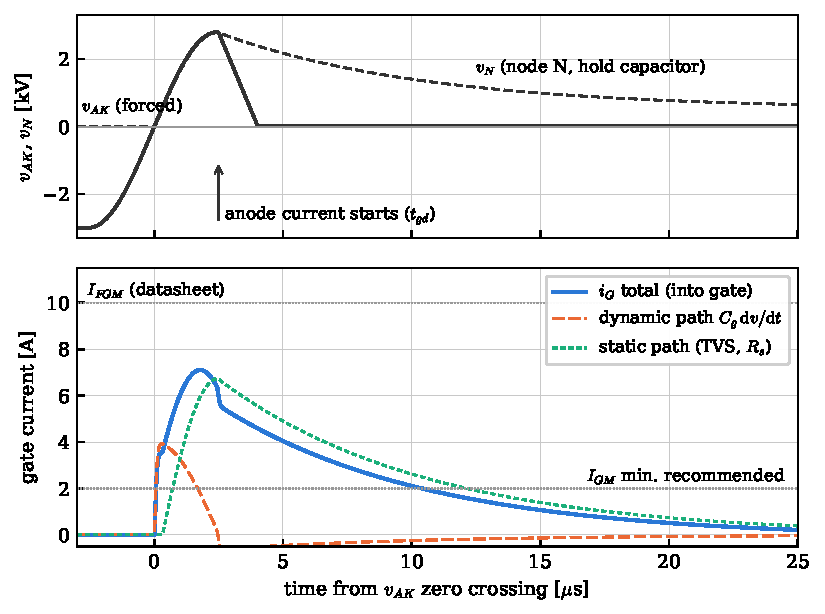
\includegraphics[width=0.9\textwidth]{gate_response.pdf}
\caption{Computed response of the gate network to the breaker opening (nominal case,
Table~\ref{tab:gate}). Top: forced anode voltage and voltage of node N. Bottom: gate current
and its two components; the static path, fed by $C_h$, sustains the pulse after the anode
voltage has collapsed.}
\label{fig:response}
\end{figure}

The nominal case gives a total gate current above the trigger level \SI{30}{ns} after the zero
crossing, above \SI{5}{A} from \SI{0.7}{\micro s}, a peak of \SI{7.1}{A} at \SI{1.8}{\micro s}
($v_{GK} \approx \SI{6}{V}$), above \SI{2}{A} until \SI{10.4}{\micro s} and above \SI{0.6}{A} until
\SI{18.3}{\micro s}; the gate charge is \SI{54}{\micro C}. Table~\ref{tab:sens} summarises the
sensitivity to the edge rate, to the MOV tolerance and to the presence of $C_h$: the limit
$I_{FGM}$ is reached only for an edge of about \SI{4}{kV/\micro s}, outside the design space
(Sec.~\ref{sec:dvdt}); without $C_h$ the pulse ends with the collapse of the anode voltage,
\SI{2.6}{\micro s} after its start, and fails the \SIrange{5}{20}{\micro s} recommendation.

\begin{table}[htbp]
\centering
\caption{Sensitivity of the computed gate pulse (network of Table~\ref{tab:gate}).}
\label{tab:sens}
\begin{tabular}{@{}lccccc@{}}
\toprule
Case & $\hat{\imath}_G$ & $\hat{\imath}_{Cg}$ & $\hat{\imath}_{D1}$ & $i_G > \SI{2}{A}$ & $i_G > \SI{0.6}{A}$ \\
\midrule
Nominal, \SI{1.8}{kV/\micro s}, plateau \SI{2.5}{kV} & \SI{7.1}{A} & \SI{3.9}{A} & \SI{43}{A} & \SI{10.3}{\micro s} & \SI{18.3}{\micro s} \\
Fast edge, \SI{3.0}{kV/\micro s} & \SI{8.5}{A} & \SI{6.4}{A} & \SI{72}{A} & \SI{9.7}{\micro s} & \SI{17.6}{\micro s} \\
Very fast edge, \SI{4.5}{kV/\micro s} & \SI{10.9}{A} & \SI{9.3}{A} & \SI{106}{A} & \SI{9.5}{\micro s} & \SI{17.5}{\micro s} \\
MOV \SI{-10}{\percent}, plateau \SI{2.0}{kV} & \SI{5.6}{A} & \SI{3.5}{A} & \SI{39}{A} & \SI{8.2}{\micro s} & \SI{16.1}{\micro s} \\
Nominal without $C_h$ & \SI{7.5}{A} & \SI{4.2}{A} & \SI{17}{A} & \SI{2.6}{\micro s} & \SI{2.8}{\micro s} \\
\bottomrule
\end{tabular}
\end{table}

\subsection{Slow reversal of the load voltage}
\label{sec:slow}

If the interruption upstream is not the IGBT breaker but a slow device -- a mechanical breaker
or a fuse -- the load voltage reverses only when the arc voltage exceeds the source voltage,
$u_{\mathrm{load}} = V_s - v_{\mathrm{arc}}$, and it does so at a rate of volts per microsecond or
less. The dynamic path is then below its \SI{300}{V/\micro s} threshold and the static path
fires the crowbar at $v_{AK} = V_{\mathrm{fire}} \approx \SI{0.75}{kV}$, i.e.\ at
$v_{\mathrm{arc}} \approx \SI{3.75}{kV}$. The commutation into $L_c$ is then driven by
$V_{\mathrm{fire}}$ only: $\mathrm{d}i/\mathrm{d}t \approx \SI{60}{A/\micro s}$,
$t_{\mathrm{comm}} \approx \SI{60}{\micro s}$, during which the arc voltage holds $v_{AK}$ near
$V_{\mathrm{fire}}$ and the static path keeps supplying \SIrange{0.7}{2}{A}; $C_h$ is charged to
$V_{\mathrm{fire}}$ only and adds little. A soft turn-on at \SI{60}{A/\micro s} with
\SI{1}{A} of gate current is within the rating conditions. This case does not size the network;
it only shows that the crowbar also protects the bench against an upstream interruption that
is not the static switch, provided the interrupting device can generate the arc voltage.

\subsection{Energy and dissipation per event}

Per opening the network handles: $\tfrac12 C_h v_{pk}^2 \approx \SI{86}{mJ}$ (of which about
\SI{30}{mJ} in the TVS stack, \SI{50}{mJ} in $R_s$, \SIrange{3}{5}{mJ} in $R_C$),
$\tfrac12 C_g v_{pk}^2 \approx \SI{9}{mJ}$ (in $R_{gs}$, the gate and $R_C$), and the gate
itself receives \SI{54}{\micro C} at \SIrange{3}{6}{V}, about \SI{0.3}{mJ}. The total is
\SI{0.1}{J} per event, i.e.\ \SI{0.1}{W} average at one opening per second: component ratings
are set by pulse voltage and pulse current, not by power.

\subsection{Failure modes and supervision}
\label{sec:fmea}

\begin{table}[htbp]
\centering
\caption{Failure modes of the network. ``Crowbar lost'' means that the MOV bank absorbs the
full \SI{16.6}{kJ} (Fig.~\ref{fig:uload}); the thyristor itself is not endangered in any case.}
\label{tab:fmea}
\begin{tabular}{@{}lp{6.2cm}p{5.4cm}@{}}
\toprule
Failure & Effect & Consequence / detection \\
\midrule
$D_1$ open & No trigger at all. & Crowbar lost; detected by plateau supervision. \\
$D_1$ short & Network exposed to \SI{-3}{kV} in service: $D_{GK}$ clamps the gate at
   \SI{-0.7}{V}; $R_s$ (\SI{27}{kW}) and $R_C$ (\SI{410}{W}) overloaded and open. & Thyristor
   safe; network destroyed, crowbar lost at the next event; \SI{8}{kV} string rating makes the
   fault remote. \\
TVS open & Dynamic path only; no sustaining current after the collapse. & Firing probable but
   outside the gate recommendations; detect with the gate-lead current transformer. \\
TVS short & Static path becomes $R_s$ from N to the gate: fires at $v_{AK} \approx \SI{0.2}{kV}$. &
   Still functional; lower threshold. \\
$C_h$ short & Node~N shorted to K: both paths disabled. & Crowbar lost; detected by plateau supervision. \\
$C_g$ short (one of two) & $C_g \to \SI{4.7}{nF}$: \SI{8.5}{A} at \SI{1.8}{kV/\micro s}. & Still
   below $I_{FGM}$; this is why $C_g$ is two capacitors in series. \\
$R_{gs}$ open & Dynamic path lost; static path unaffected. & Functional. \\
\bottomrule
\end{tabular}
\end{table}

The failure modes that lose the crowbar all show up in the load voltage: the plateau at
\SI{-2.5}{kV} lasts about \SI{20}{\micro s} when the crowbar works and about \SI{2}{ms} when it
does not (Fig.~\ref{fig:uload}). A supervision rule in the bench controller -- alarm and stop
if $u_{\mathrm{load}} < \SI{-1}{kV}$ persists for more than \SI{100}{\micro s} -- protects the MOV
bank against a silent loss of the crowbar. The gate-lead current transformer allows the pulse
of Fig.~\ref{fig:response} to be checked at commissioning and periodically.

\subsection{Optional active trigger}

If the breaker controller can issue a gate command, it should be used as the primary trigger
(pulse transformer or fibre-optic gate unit) with the passive network of Fig.~\ref{fig:gate} left
in place as an independent back-up -- the same philosophy as HVDC valves. The command must be
issued together with, not before, the IGBT turn-off: a positive gate pulse applied while the
thyristor still blocks \SI{-3}{kV} produces the reverse-leakage amplification described in
Sec.~\ref{sec:network}. With an active unit the passive network is unchanged; the two pulses
simply add at the gate, and the sum must still respect $I_{FGM}$.

% ==========================================================================
\section{Coordination with the MOV clamp}
% ==========================================================================

\begin{enumerate}
\item \textbf{Firing level:} $V_{\mathrm{fire}} \ll V_{\mathrm{MOV}} - V_s$. With
      $V_{\mathrm{fire}} \approx \SI{0.75}{kV}$ and \SIrange{2.0}{2.8}{kV} available the margin
      is a factor \numrange{2.7}{3.7}; the dynamic path fires at the zero crossing.
\item \textbf{$\mathrm{d}i/\mathrm{d}t$:} $(V_{\mathrm{MOV}} - V_s)/L_c = \SIrange{200}{224}{A/\micro s}$,
      independent of the trigger; equal to the \SI{50}{Hz} rating, five times below the
      \SI{1}{Hz} rating, with a gate pulse three times the rating conditions. The two
      knobs are $L_c$ and the MOV clamp level (Secs.~\ref{sec:lc} and \ref{sec:didt}).
\item \textbf{MOV duty:} about \SI{180}{J} per opening during the \SI{20}{\micro s} of gate delay
      and commutation; the varistor bank becomes a back-up clamp with negligible ageing.
\item \textbf{MOV tolerance:} the network works from a plateau of \SI{2.0}{kV} upwards
      (Table~\ref{tab:sens}); a lower clamp level, if ever chosen to reduce the
      $\mathrm{d}i/\mathrm{d}t$, requires re-checking the sustaining current or lowering $V_{st}$.
\item \textbf{Branch snubber:} at firing $C_{sn}$ discharges through $R_{sn}$ into the thyristor,
      $v_{AK}/R_{sn} \le \SI{44}{A}$ and $\tfrac12 C_{sn} v_{AK}^2 \le \SI{8}{J}$ in $R_{sn}$:
      harmless.
\end{enumerate}

% ==========================================================================
\section{Verification in simulation}
\label{sec:verif}
% ==========================================================================

With the existing Simscape model of the 5STP~26N6500 and the gate network of
Table~\ref{tab:gate} added:

\begin{itemize}
\item Plot $v_{AK}$ (device terminals, not branch voltage), $i_G$, $v_{GK}$, $i_{D1}$ and $i_A$
      at breaker opening. Confirm that $i_G$ exceeds $I_{GT}$ while $v_{AK}$ is still low, that
      the peak of $i_G$ stays below \SI{10}{A}, that $i_G > \SI{2}{A}$ for at least
      \SI{5}{\micro s} after the anode voltage has collapsed, and record the forward voltage at
      which anode current starts. Compare with Fig.~\ref{fig:response}.
\item Confirm the load-voltage waveform of Sec.~\ref{sec:meaning}: plateau of about
      \SI{20}{\micro s}, then $\approx \SI{-1.5}{kV}$ decaying with \SI{1.64}{ms}; MOV energy
      $\approx \SI{180}{J}$.
\item Extract $\mathrm{d}i_A/\mathrm{d}t$ during the first \SI{20}{\micro s} and compare with the
      repetitive rating; evaluate $L_c = \SIrange{15}{18}{\micro H}$ if margin is wanted on the
      \SI{50}{Hz} figure.
\item Sweep the breaker edge rate from \SI{0.3}{kV/\micro s} to \SI{3}{kV/\micro s} (breaker
      snubber capacitance, IGBT gate resistance) and the MOV clamp level by $\pm\SI{10}{\percent}$;
      the static path should take over below the threshold \eqref{eq:dvth} and the sustaining
      current should remain above \SI{4}{A} on the plateau.
\item Breaker closing: $v_{AK}$ steps from \SI{0}{} to \SI{-3}{kV}; check that the gate stays
      quiet ($v_{GK}$ within \SI{\pm 1}{V}), that node~N does not move by more than a few volts,
      and that $D_1$ sees no overvoltage beyond its rating including the closing overshoot.
\item Abnormal case: breaker re-closing, or reconnection of the low-voltage pre-heating source,
      while the crowbar still conducts. The source then forces the crowbar current to zero
      through $L_c$ (\SI{240}{A/\micro s} at \SI{3}{kV}, \SI{4}{A/\micro s} at \SI{50}{V}) with
      reverse recovery; check the reverse voltage overshoot across $T$ and the branch snubber. The
      turn-off time $t_q = \SI{800}{\micro s}$ is irrelevant in normal operation, since forward
      voltage returns only at the next cycle.
\item Slow opening (Sec.~\ref{sec:slow}): ramp $v_{AK}$ at \SI{10}{V/\micro s} and confirm firing
      at $\approx V_{\mathrm{fire}}$ with the anode current rising at \SI{60}{A/\micro s}.
\end{itemize}

% ==========================================================================
\section{Conclusions}
% ==========================================================================

The crowbar thyristor of the \SI{3}{kV} / \SI{3600}{A} bench dissipates about \SI{10}{J} per
event and is sized by voltage, $\mathrm{d}i/\mathrm{d}t$ and cycle count. A symmetric
\SI{6.5}{kV} phase-control thyristor such as the 5STP~26N6500 is the appropriate choice: it
blocks the \SI{3}{kV} reverse DC of service life with adequate cosmic-ray margin, and its
$\mathrm{d}i/\mathrm{d}t$ capability matches the \SIrange{200}{224}{A/\micro s} imposed by $L_c$
and the MOV clamp. That $\mathrm{d}i/\mathrm{d}t$ is set by the dump inductor and not by the load
inductance: during the transfer of the current from the varistor to the thyristor the \SI{2}{mH}
act as a constant current source, and the transfer rate is
$(V_{\mathrm{MOV}} - V_s)/(L_c + L_\sigma)$ -- without $L_c$ it would be the kiloampere-per-microsecond
figure of the bus-bar stray inductance. $L_c$ is the trade-off between the thyristor
$\mathrm{d}i/\mathrm{d}t$ and the MOV energy per event.

The simulated load voltage at breaker opening -- a swing from $+\SI{3}{kV}$ to \SI{-2.8}{kV} in
\SIrange{4}{5}{\micro s}, a plateau at \SI{-2.5}{kV} and, without crowbar, \SI{2}{ms} of MOV
conduction with \SI{16.6}{kJ} -- shows that the intrinsic self-firing mechanisms cannot be relied
upon: forward breakover is unreachable and the $\mathrm{d}v/\mathrm{d}t$ of \SIrange{1.5}{2}{kV/\micro s}
is below the critical \SI{3}{kV/\micro s}, so the device would simply block. A negative load
voltage is, in this DC circuit with unidirectional current, an unambiguous signal that the path
from the source has been interrupted, and the trigger network is designed to respond to it and to
nothing else: the blocking diode $D_1$ keeps the network inert for $u_{\mathrm{load}} > 0$, the
coupling capacitor fires the gate at the zero crossing of the load voltage, the TVS stack with its
series resistor fires it at $u_{\mathrm{load}} \approx \SI{-0.75}{kV}$ on any slow reversal and
sustains \SIrange{5}{7}{A} on the MOV plateau, and the hold capacitor extends the pulse to
\SIrange{10}{18}{\micro s} after the anode voltage has collapsed, in line with the gate-drive
recommendations of the manufacturer. The design values of Table~\ref{tab:gate} respect
$I_{FGM}$ and $V_{RGM}$ with margin, handle about \SI{0.1}{J} per event, and fail either safe or
detectably; a supervision of the plateau duration in the bench controller and a current
transformer on the gate lead complete the scheme. Firing level and $\mathrm{d}i/\mathrm{d}t$ are
coordinated with the MOV clamp through $V_{\mathrm{fire}} \ll V_{\mathrm{MOV}} - V_s$ and
$(V_{\mathrm{MOV}} - V_s)/L_c$.

% ==========================================================================
\begin{thebibliography}{9}

\bibitem{ds26n6500}
Hitachi Energy (formerly ABB Semiconductors), ``Phase Control Thyristor 5STP~26N6500,'' data sheet.

\bibitem{an5sya2034}
ABB Switzerland Ltd, Semiconductors, ``Gate-drive recommendations for phase control thyristors,''
Application Note 5SYA~2034.

\bibitem{baliga}
B.~J. Baliga, \emph{Fundamentals of Power Semiconductor Devices}. New York: Springer, 2008,
ch.~8 (Thyristors).

\bibitem{bodpatent}
``Protective circuitry for a thyristor,'' U.S. Patent 4\,651\,251 (break-over diode protective firing, Nelson River HVDC precedent).

\bibitem{arrillaga}
J.~Arrillaga, \emph{High Voltage Direct Current Transmission}, 2nd ed. London: IEE, 1998
(thyristor valves, protective firing).

\bibitem{dynexpp}
Dynex Semiconductor, ``Pulsed power thyristors,'' product information, accessed Sept.~2026.

\bibitem{tvs5kp}
Littelfuse / Vishay, ``5KP series -- 5000~W transient voltage suppressors,'' data sheet.

\bibitem{abbsnubber}
ABB Switzerland Ltd, Semiconductors, ``Design of RC snubbers for phase control applications,''
Application Note 5SYA~2020.

\end{thebibliography}

\end{document}
